\section{SENSORES - Sensor de luz ambiental}

% DONE: Simulacion

En esta experiencia de laboratorio, se desarrollará un sistema de medición ambiental utilizando los siguientes componentes: 
\begin{itemize}
    \item 1 LDR (sensor de luz)
    \item Diodos LED
    \item Buzzer (alarma)
    \item Botón o switch
\end{itemize}

El objetivo de esta experiencia es implementar un sistema que permita medir la cantidad de luz en un ambiente determinado, el cual complementaría (idealmente) un sistema de cámaras de seguridad y un control inteligente de iluminación. El sistema debe cumplir con las siguientes funciones:
\begin{enumerate}
    \item Cuando el nivel de iluminación es bajo, los focos de la habitación deben encenderse, representado por el encendido de un LED rojo.
    \item Cuando el nivel de iluminación es alto, los focos deben permanecer apagadas, representado por el LED rojo apagado.
    \item Las cámaras de seguridad deben estar en funcionamiento en todo momento, lo cual se representa mediante el encendido de un LED azul.
    \item En caso de que no se detecte energía eléctrica para el sistema de cámaras (entrada digital detecta GND), el sistema debe encender y apagar el LED azul de manera intermitente, además de activar un buzzer que representa una alarma de error. Esto puede simularse utilizando un botón, un switch o una desconexión de cable.
\end{enumerate}

La implementación se realizó en la plataforma Tinkercad, utilizando un Arduino UNO. La conexión de los componentes se puede observar en la Figura \ref{fig:luz_ambiental}. El sensor LDR se conectó a una entrada analógica (A0), mientras que los LEDs y el buzzer se conectaron a salidas digitales. Un botón se empleó como entrada digital para simular la presencia o ausencia de energía del sistema de cámaras.

\begin{figure}[H]
    \centering
    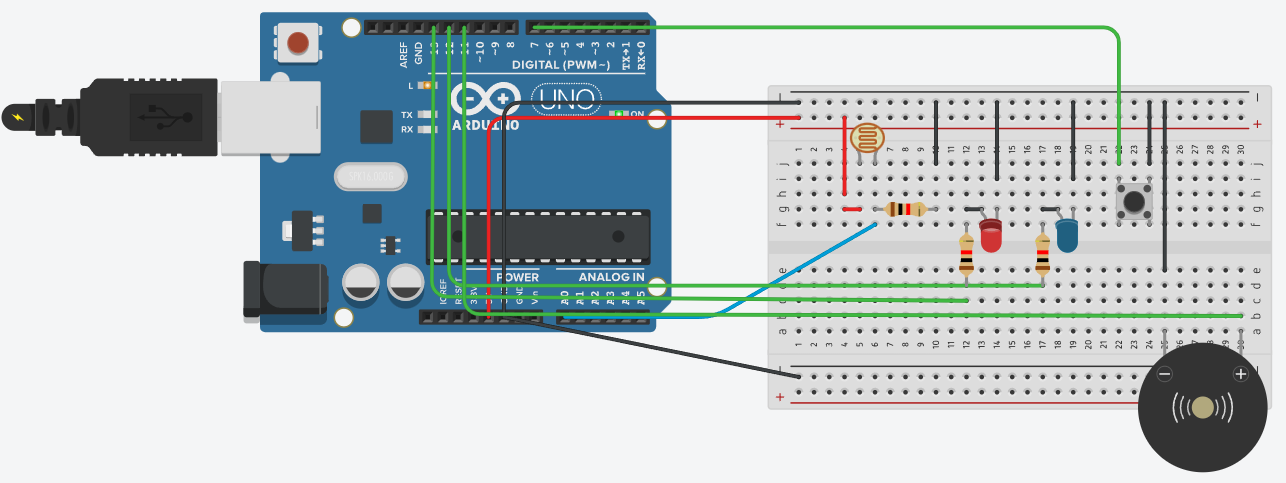
\includegraphics[width=0.85\textwidth]{./img/ckpt_1.png}
    \caption{Simulación Tinkercad Sensor de luz ambiental}
    \label{fig:luz_ambiental}
\end{figure}

En el código (Código \ref{code:sensor_ambiental}), se define un umbral de luminosidad para distinguir entre un ambiente claro u oscuro. Si el valor leído del LDR es menor que este umbral, se activa el LED rojo. Por otro lado, si el botón indica que hay energía (estado HIGH), el LED azul permanece encendido de forma constante. En caso contrario (estado LOW), el sistema simula una falla eléctrica encendiendo el buzzer y haciendo parpadear el LED azul.

\begin{lstlisting}[style=cppstyle, caption={Código en C++ para el sensor ambiental.}, label={code:sensor_ambiental}]
int LDR_pin = A0;
int ROJO_pin = 13;
int AZUL_pin = 12;
int BUZZER_pin = 11;
int BUTTON_pin = 7;
int luz, estadoBoton;
const int umbral = 500;  // Ajustarlo

void setup() {
    pinMode(ROJO_pin, OUTPUT); pinMode(AZUL_pin, OUTPUT);
    pinMode(BUZZER_pin, OUTPUT);
    pinMode(BUTTON_pin, INPUT_PULLUP);
    Serial.begin(9600);
}

void loop() {
    luz = analogRead(LDR_pin);
    estadoBoton = digitalRead(BUTTON_pin);
    Serial.println("Luz: " + String(luz) + " - " + String(umbral));
    
    if (luz < umbral) digitalWrite(ROJO_pin, HIGH);
    else digitalWrite(ROJO_pin, LOW);
    
    if (estadoBoton == HIGH) {
        digitalWrite(AZUL_pin, HIGH);
        digitalWrite(BUZZER_pin, LOW);
    } else {
        digitalWrite(BUZZER_pin, HIGH);
        digitalWrite(AZUL_pin, HIGH); delay(300);
        digitalWrite(AZUL_pin, LOW); delay(300);
    }
    delay(1000);
}    
\end{lstlisting}

\begin{figure}[H]
    \centering
    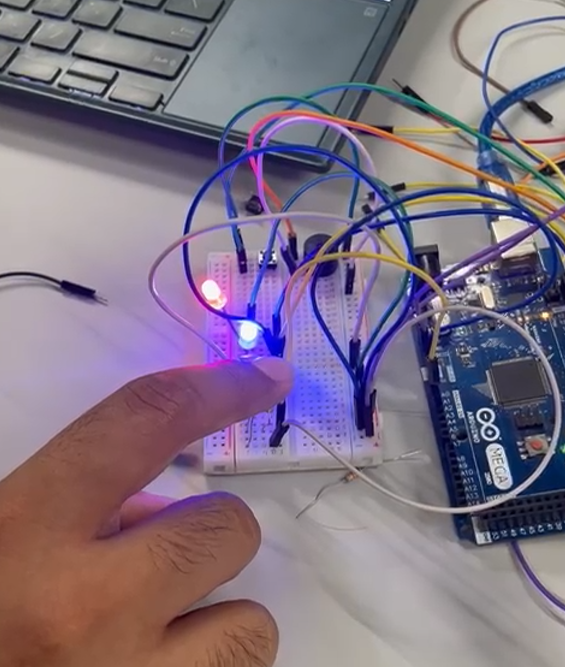
\includegraphics[width=0.5\textwidth]{img/sensores_chkp_2.png}
    \caption{Implementación en laboratorio: Estado de luz baja (LED rojo encendido) y camáras en funcionamiento (LED azul encendido)}
    \label{fig:luz_ambiental_lab_estado_1}
\end{figure}


\begin{figure}[H]
    \centering
    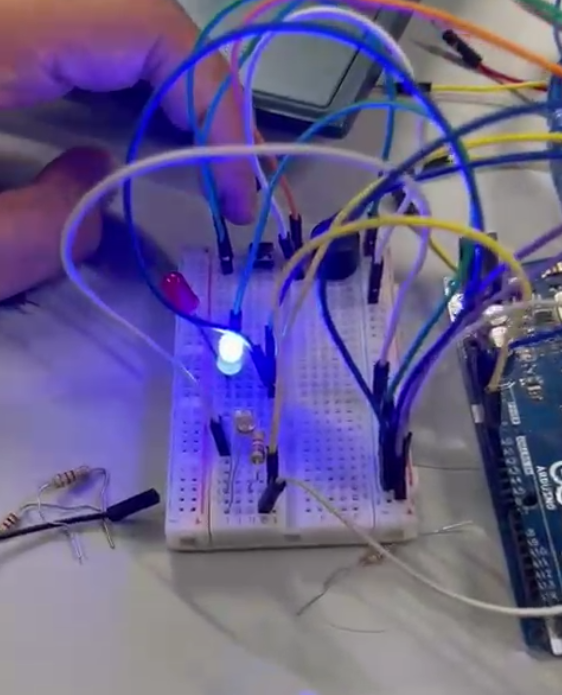
\includegraphics[width=0.5\textwidth]{img/sensores_chkp_2_2.png}
    \caption{Implementación en laboratorio: Estado de funcionamiento (LED rojo apagado) y camáras en funcionamiento (LED azul encendido)}
    \label{fig:luz_ambiental_lab_estado_2}
\end{figure}

\begin{figure}[H]
    \centering
    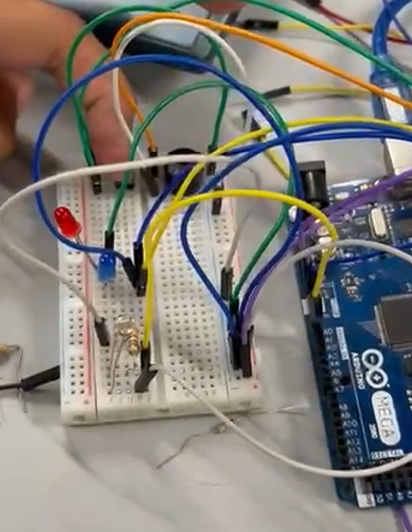
\includegraphics[width=0.5\textwidth]{img/sensores_chkp_2_1.png}
    \caption{Implementación en laboratorio: Estado de corte de energía/error (buzzer activo)}
    \label{fig:luz_ambiental_lab_estado_3}
\end{figure}

% Enlace al video: \url{https://drive.google.com/file/d/1v76hk4pJjSoHVMHp4mmkme9ZRFEXyfd-/view}

% DONE: foto de la implementacion presencial en el laboratorio

\section{SENSORES - Cerradura inteligente}

% TODO: Diagrama de flujo
% DONE: Simulacion
En esta experiencia de laboratorio, se desarrollará un sistema de seguridad para el control de acceso de personas a un área restringida. Para ello, se utilizarán los siguientes componentes: 

\begin{itemize}
    \item 01 sensor de proximidad.
    \item 01 teclado matricial.
    \item 01 LCD 2x16.
    \item Diodos LED.
    \item Resistencias variadas.
    \item Jumpers.
\end{itemize}
% TODO: foto de la implementacion presencial en el laboratorio
A continuación, se presenta la simulación del sistema de cerradura inteligente en Tinkercad. Se desglosa la implementacion en cuatro partes:
\begin{itemize}
    \item Presencia de la persona.
    \item Mensaje en LCD.
    \item Autenticación.
    \item Ahorro energético (Standby).
\end{itemize}
\subsection{Presencia de la persona}
El primer paso de la simulación consiste en detectar la presencia de una persona utilizando un sensor de proximidad. Este sensor se conecta a un pin digital del Arduino y se utiliza para encender un LED rojo cuando se detecta movimiento. La simulación se puede observar en la Figura \ref{fig:cerradura_smart_presencia}.
\begin{figure}[H]
    \centering
    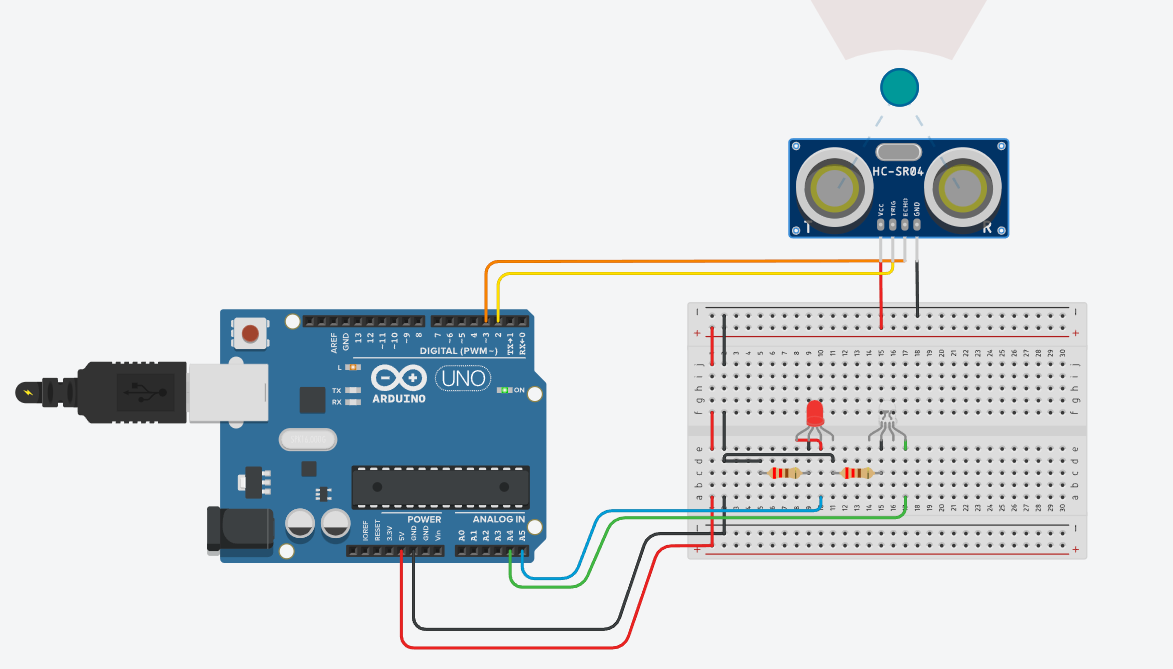
\includegraphics[width=0.85\textwidth]{./img/2-1-presencia-de-persona.png}
    \caption{Simulación Tinkercad integrando el sensor de proximidad al sistema de cerradura inteligente}
    \label{fig:cerradura_smart_presencia}
\end{figure}

\subsection{Mensaje en LCD}
El segundo paso consiste en mostrar un mensaje en un LCD 2x16 cuando se detecta la presencia de una persona. El mensaje indica que el sistema está esperando la autenticación. La simulación se puede observar en la Figura \ref{fig:cerradura_smart_LCD}.
El LCD se conecta a los pines digitales del Arduino y se utiliza la biblioteca LiquidCrystal para controlar su funcionamiento. El código de la simulación se puede observar en el Código \ref{code:cerradura_smart_LCD}.
\begin{figure}[H]
    \centering
    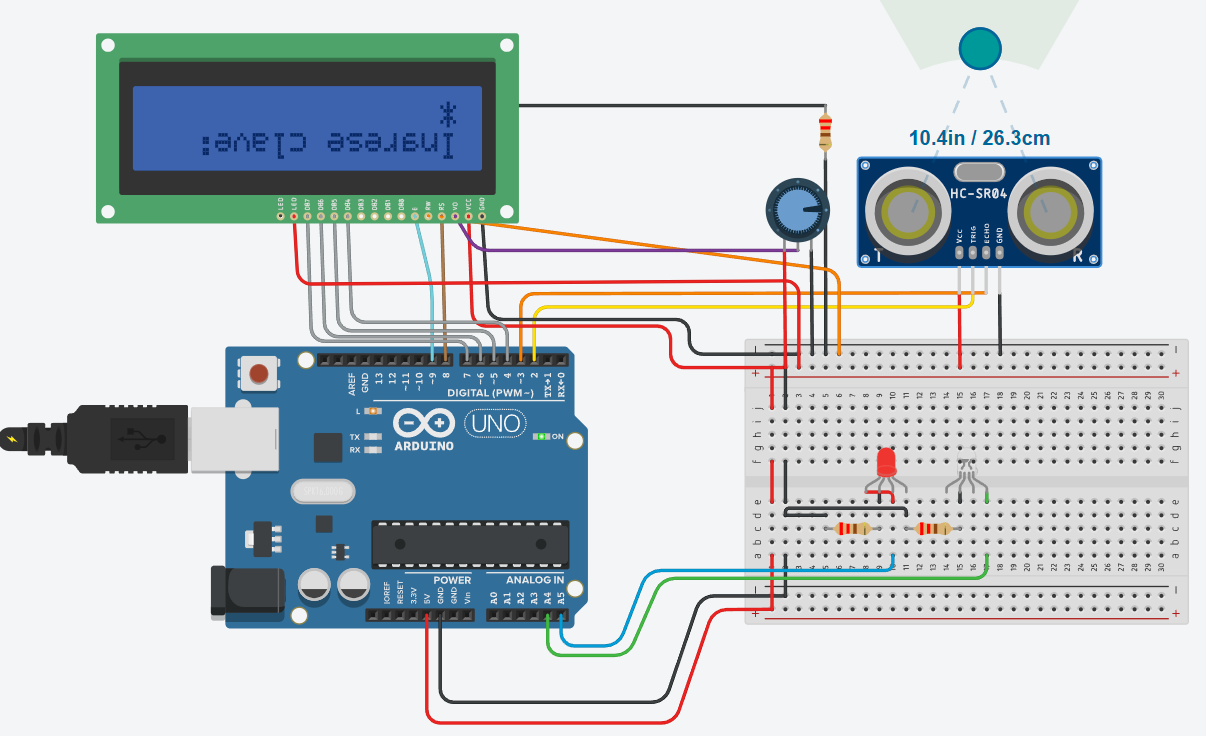
\includegraphics[width=0.85\textwidth]{./img/2-2-Mensaje-LCD.png}
    \caption{Simulación Tinkercad integrando LCD al sistema de cerradura inteligente}
    \label{fig:cerradura_smart_LCD}
\end{figure}

\subsection{Autenticación}
El tercer paso consiste en implementar un sistema de autenticación utilizando un teclado matricial. El usuario debe ingresar un código de acceso para desbloquear la cerradura. Si el código es correcto, se enciende un LED verde y se muestra un mensaje de "Acceso correcto" en el LCD. Si el código es incorrecto, se enciende un LED rojo y se muestra un mensaje de "Clave Incorrecta". La simulación se puede observar en la Figura \ref{fig:cerradura_smart_autenticacion}.
El teclado matricial se conecta a los pines digitales del Arduino y se utiliza la biblioteca Keypad para controlar su funcionamiento. El código de la simulación se puede observar en el Código \ref{code:cerradura_smart_LCD}.
\begin{figure}[H]
    \centering
    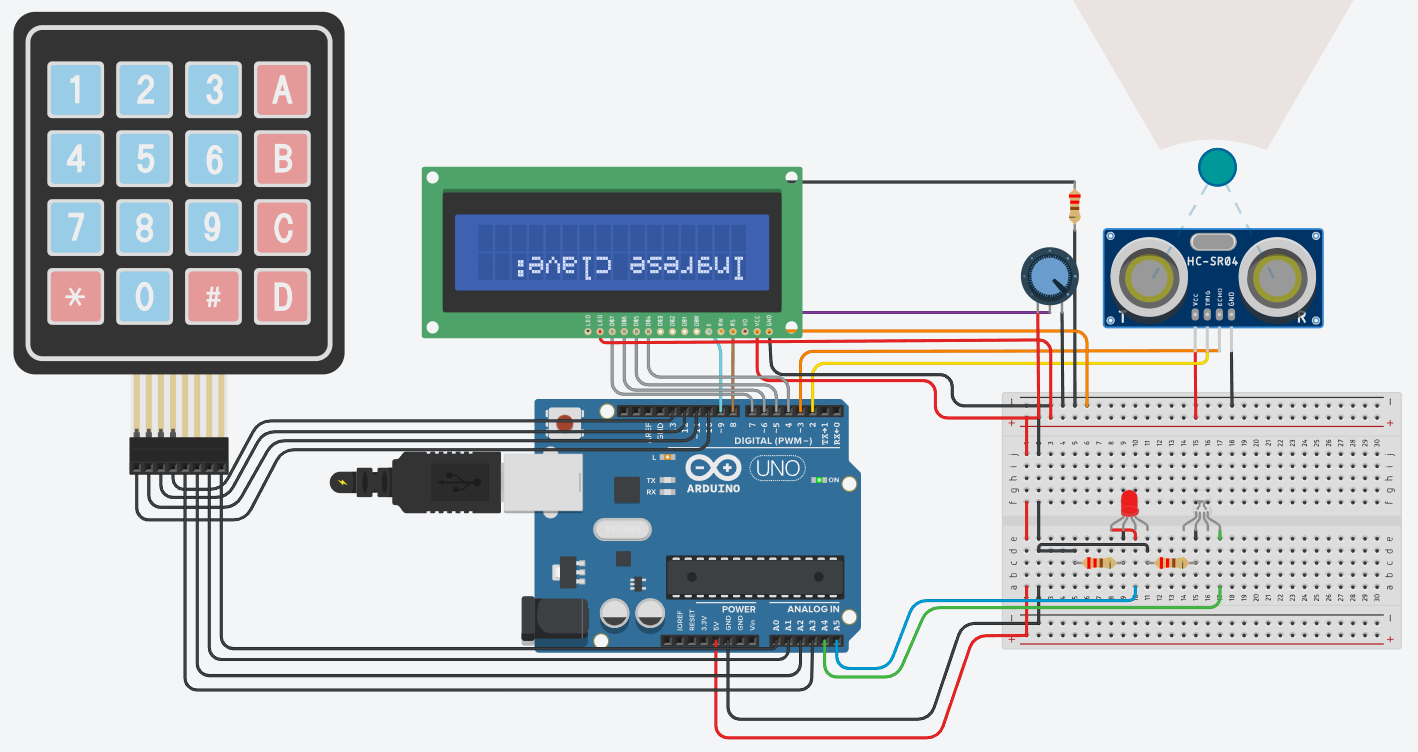
\includegraphics[width=0.85\textwidth]{./img/2-3-Autenticacion.png}
    \caption{Simulación Tinkercad Aplicando la autenticación}
    \label{fig:cerradura_smart_autenticacion}
\end{figure}

\subsection{Ahorro Energético (Standby)}
El cuarto paso consiste en implementar un sistema de ahorro energético. Cuando no se detecta movimiento durante un período de tiempo determinado, el sistema entra en modo de espera (standby) y apaga el LCD y los LEDs. La simulación se puede observar en la Figura \ref{fig:cerradura_smart_final}. Finalmente, se puede observar el diagrama de flujo del sistema de cerradura inteligente en la Figura \ref{fig:flujo_cerradura_smart}. El diagrama muestra el flujo de trabajo del sistema, desde la detección de movimiento hasta la autenticación y el ahorro energético.
\begin{figure}[H]
    \centering
    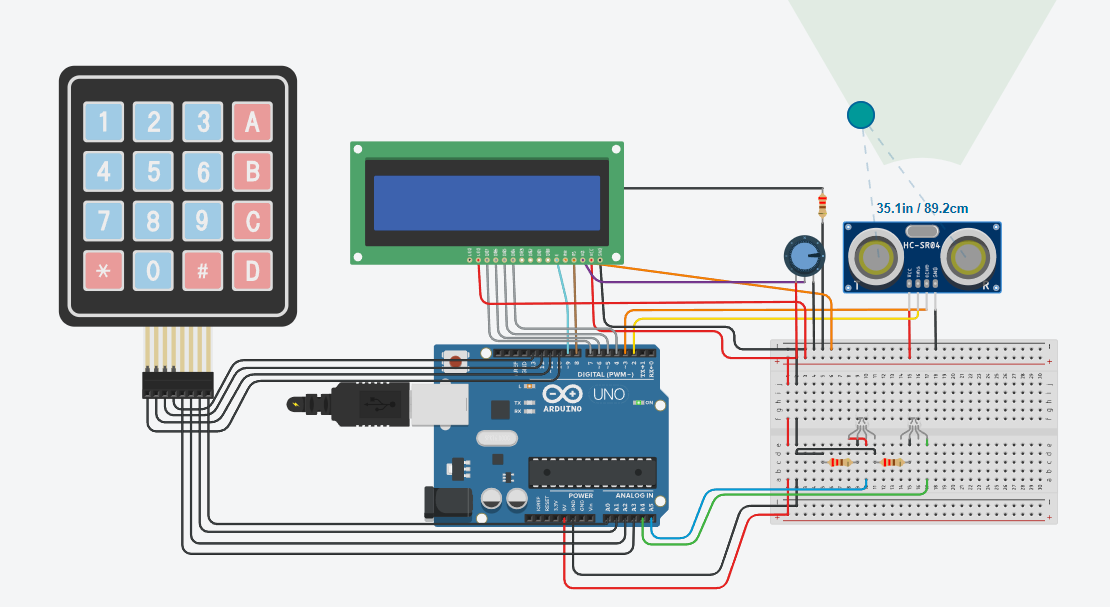
\includegraphics[width=0.85\textwidth]{./img/2-4-Ahorro-energetico.png}
    \caption{Simulación Tinkercad Resultado final del sistema de cerradura inteligente}
    \label{fig:cerradura_smart_final}
\end{figure}

\begin{figure}[H]
    \centering
    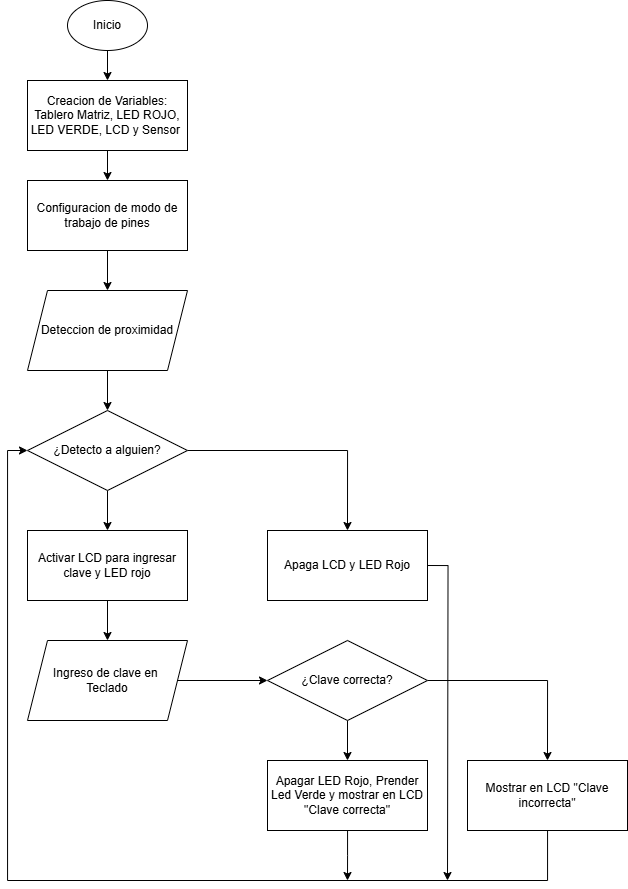
\includegraphics[width=0.7\textwidth]{./img/2-Diagrama-flujo.png}
    \caption{Diagrama de flujo del sistema de cerradura inteligente}
    \label{fig:flujo_cerradura_smart}
\end{figure}

\begin{lstlisting}[style=cppstyle, caption={Código en C++ para el sistema de control de aforo.}, label={code:cerradura_smart_LCD}]
#include <LiquidCrystal.h>
#include <Keypad.h>

// Configuracion del LCD
LiquidCrystal lcd(8, 9, 4, 5, 6, 7);

// Configuracion del sensor ultrasonico
const int triggerPin = 2;
const int echoPin = 3;

// Configuracion de LEDs
const int ledRojo = A5;
const int ledVerde = A4;

// Contrasenha correcta
String password = "1234";
String inputPassword = "";

// Configuracion del Keypad
const byte ROWS = 4; // 4 filas
const byte COLS = 4; // 4 columnas

char keys[ROWS][COLS] = {
  {'1','2','3','A'},
  {'4','5','6','B'},
  {'7','8','9','C'},
  {'*','0','#','D'}
};

// Ajustar pines del keypad segun tu tabla
byte rowPins[ROWS] = {10, 11, 12, 13}; // Filas
byte colPins[COLS] = {A3, A2, A1, A0}; // Columnas

Keypad keypad = Keypad(makeKeymap(keys), rowPins, colPins, ROWS, COLS);

void setup() {
  Serial.begin(9600);
  
  pinMode(triggerPin, OUTPUT);
  pinMode(echoPin, INPUT);
  pinMode(ledRojo, OUTPUT);
  pinMode(ledVerde, OUTPUT);
  
  lcd.begin(16, 2);
  lcd.clear();
}

void loop() {
  long distance = getDistance();

  if (distance < 20) {
    digitalWrite(ledRojo, HIGH); // Activar grabacion (presencia detectada)
    lcd.clear();
    lcd.setCursor(0, 0);
    lcd.print("Ingrese clave:");
    inputPassword = "";

    while (inputPassword.length() < 4) {
      char key = keypad.getKey();
      if (key) {
        inputPassword += key;
        lcd.setCursor(inputPassword.length() - 1, 1);
        lcd.print("*"); // Mostrar asterisco por cada numero
      }
    }

    delay(500);
    lcd.clear();
    
    if (inputPassword == password) {
      lcd.setCursor(0, 0);
      lcd.print("Acceso correcto");
      digitalWrite(ledRojo, LOW);
      digitalWrite(ledVerde, HIGH);
      delay(3000);
      digitalWrite(ledVerde, LOW);
    } else {
      lcd.setCursor(0, 0);
      lcd.print("Clave incorrecta");
      delay(2000);
    }
  } else {
    digitalWrite(ledRojo, LOW); // Standby: nadie presente
    lcd.clear();
  }
}

long getDistance() {
  digitalWrite(triggerPin, LOW);
  delayMicroseconds(2);
  digitalWrite(triggerPin, HIGH);
  delayMicroseconds(10);
  digitalWrite(triggerPin, LOW);
  
  long duration = pulseIn(echoPin, HIGH);
  long distance = duration * 0.034 / 2;
  return distance;
}
\end{lstlisting}

\section{SENSORES - Sistema de control de aforo}

% DONE: Simulacion
La presente experiencia de laboratorio tiene como objetivo implementar un sistema de control de aforo utilizando un sensor PIR (Passive Infrared Sensor) y un LCD. El sistema se basa en la detección de movimiento para contar el número de personas que ingresan a un área determinada. A continuación, se describen los componentes utilizados:

\begin{itemize}
    \item Arduino
    \item Sensor PIR
    \item Diodo LED verde
    \item Diodo LED rojo
    \item LCD 2x16
\end{itemize}

\subsection{Funcionamiento}

El sensor de movimiento PIR es el encargado de detectar la presencia o movimiento de personas en la zona monitoreada. El sistema opera bajo dos modos principales, los cuales se ilustran en las Figuras \ref{fig:control_aforo_reposo} y \ref{fig:control_aforo_contando}.

\begin{enumerate}
    \item \textbf{Modo de Reposo:} Cuando no se detecta movimiento, el sistema entra en modo de reposo. En este estado, el LED verde se enciende y apaga de manera intermitente cada 200 ms, indicando que el sistema está activo y a la espera de detectar alguna incidencia. La Figura \ref{fig:control_aforo_reposo} muestra el sistema en este estado, con el LED verde parpadeando y el LCD indicando el modo de reposo.
    
    \item \textbf{Detección de Movimiento:} Al detectar movimiento en el área, el sistema apaga el LED verde y enciende el LED rojo, señalizando la presencia de una persona. Simultáneamente, el LCD muestra la cantidad de incidencias detectadas, por ejemplo: ``INCIDENCIAS 001''. Es importante destacar que el sistema implementa una lógica de temporización para evitar contar múltiples veces a la misma persona: si el movimiento persiste durante 500 ms, el contador no incrementa. Solo si, tras 5 segundos sin movimiento, se vuelve a detectar una nueva presencia, el contador incrementa nuevamente (por ejemplo, ``INCIDENCIAS 002''). La Figura \ref{fig:control_aforo_contando} ilustra el sistema durante la detección de movimiento, con el LED rojo encendido y el LCD mostrando el conteo de incidencias.
    
    \item \textbf{Retorno al modo de reposo:} Si el sistema deja de detectar movimiento, automáticamente retorna al modo de reposo, reanudando el parpadeo del LED verde y esperando nuevas incidencias.
\end{enumerate}

Para comprender la arquitectura general del sistema, se presenta el diagrama de bloques en la Figura \ref{fig:bloques_conteo_personas}, donde se visualizan las conexiones y la interacción entre los distintos componentes. El flujo lógico de funcionamiento, desde la detección de movimiento hasta el conteo y visualización en el LCD, se detalla en el diagrama de flujo de la Figura \ref{fig:flujo_conteo_personas}. Finalmente, el Código \ref{code:sensor_ambiental} muestra la implementación en Arduino, donde se observa cómo se lleva a cabo la lógica de detección, conteo y visualización, siguiendo la secuencia planteada en los diagramas mencionados.

\begin{figure}[H]
    \centering
    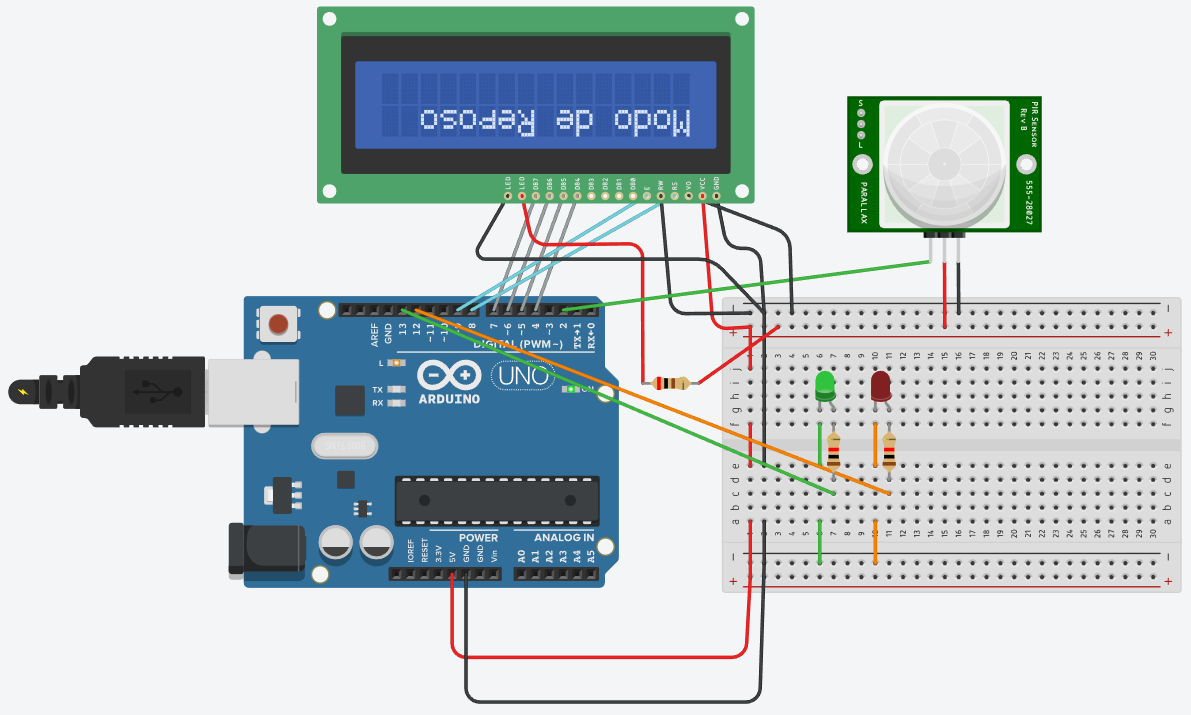
\includegraphics[width=0.85\textwidth]{./img/ckpt_9_1.png}
    \caption{Simulación Tinkercad: Estado de reposo (LED verde parpadeando, sistema activo)}
    \label{fig:control_aforo_reposo}
\end{figure}

\begin{figure}[H]
    \centering
    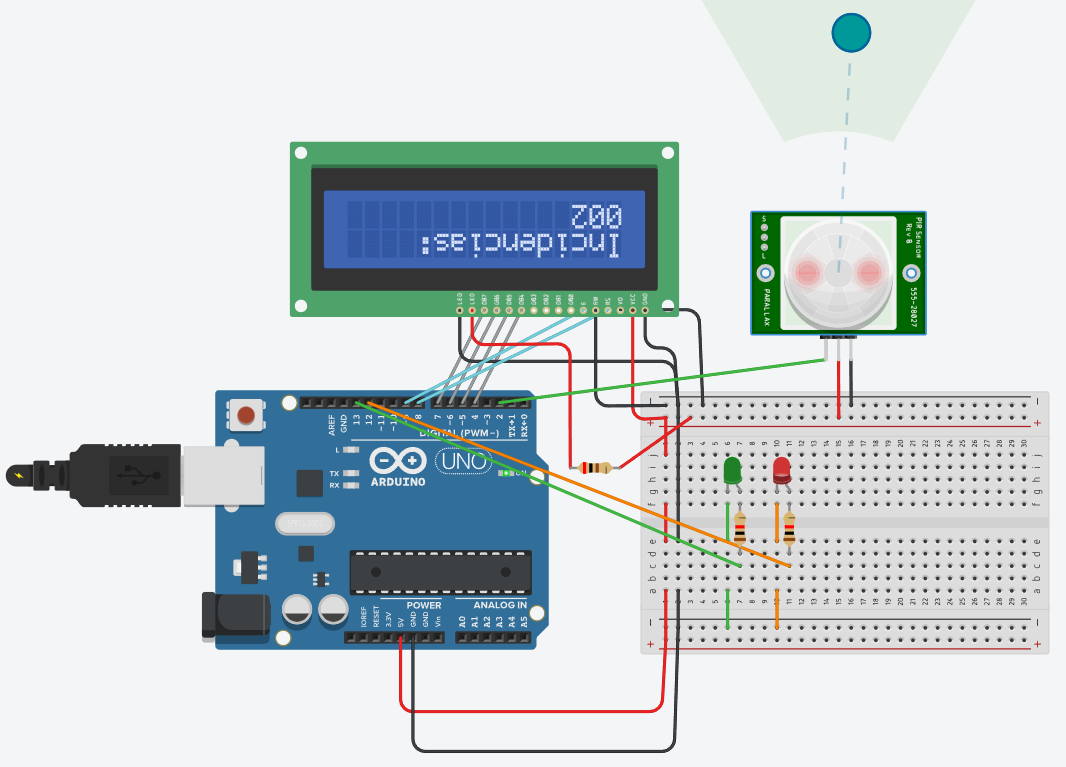
\includegraphics[width=0.85\textwidth]{./img/ckpt_9.png}
    \caption{Simulación Tinkercad: Estado de detección de movimiento (LED rojo encendido, pantalla contando incidencias)}
    \label{fig:control_aforo_contando}
\end{figure}

\begin{figure}[H]
    \centering
    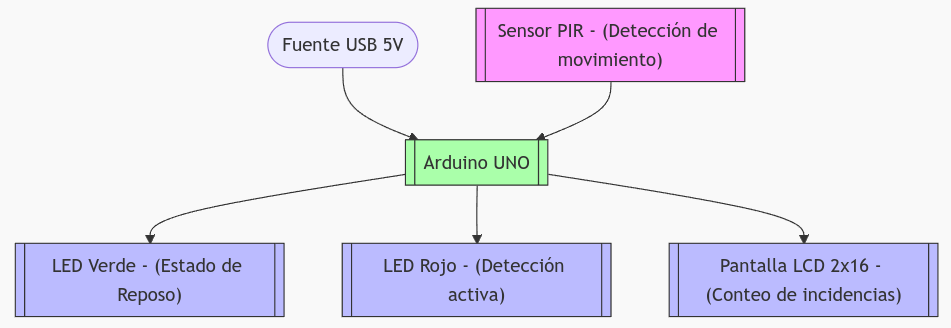
\includegraphics[width=0.85\textwidth]{./img/bloques_conteo_personas.png}
    \caption{Diagrama de bloques del sistema de control de aforo}
    \label{fig:bloques_conteo_personas}
\end{figure}

\begin{figure}[H]
    \centering
    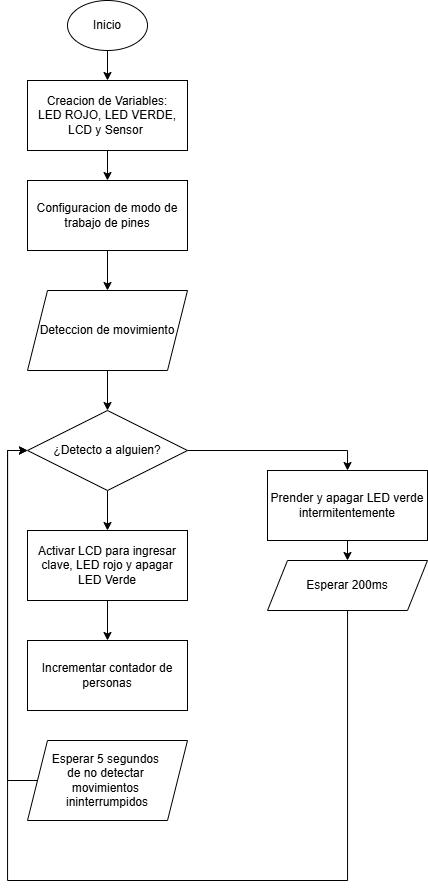
\includegraphics[width=0.5\textwidth]{./img/3-Diagrama-flujo.png}
    \caption{Diagrama de flujo del sistema de control de aforo}
    \label{fig:flujo_conteo_personas}
\end{figure}

\begin{lstlisting}[style=cppstyle, caption={Código en C++ para el sistema de control de aforo.}, label={code:sensor_ambiental}]
#include <LiquidCrystal.h>

// Configuracion del LCD
LiquidCrystal lcd(8, 9, 4, 5, 6, 7);
const int PIRPin = 2;
const int LEDGreen = 13;
const int LEDRed = 12;

// Variable to store the number of incidents
int incidentCount = 0;

void setup() {
    Serial.begin(9600);
    
    lcd.begin(16, 2);
    lcd.clear();
    pinMode(PIRPin, INPUT);
    pinMode(LEDGreen, OUTPUT);
    pinMode(LEDRed, OUTPUT);
}

void loop() {
    int value = digitalRead(PIRPin);
    Serial.println(value);

    if (value == LOW) {
    // No movement detected, indicating the rest mode
    digitalWrite(LEDGreen, HIGH);   // Green LED blink (indicates idle state)
    delay(200);
    digitalWrite(LEDGreen, LOW);
    delay(200);
    
    // Display "RESTING" on LCD when no movement detected
    lcd.clear();
    lcd.setCursor(0, 0);
    lcd.print("Modo de Reposo");
    } else {
    // Movement detected, indicating the active state
    digitalWrite(LEDGreen, LOW);    // Turn off the green LED
    digitalWrite(LEDRed, HIGH);     // Turn on the red LED

    // Increment incident count when movement is detected
    incidentCount++;

    // Display incident count on LCD
    lcd.clear();
    lcd.setCursor(0, 0);
    lcd.print("Incidencias: ");
    lcd.setCursor(0, 1);
    lcd.print("00" + String(incidentCount));  // Assuming a 3-digit max count
    
    delay(2000); // Wait 2 seconds before checking again
    }
    
    delay(10);  // Small delay to stabilize the loop
}    
\end{lstlisting}
    
% DONE: foto de la implementacion presencial en el laboratorio
% DONE: diagrama de flujo
% DONE: diagrama de bloques

% Enlace al video: \url{https://drive.google.com/file/d/1VmmF8ljH7DoGnzlM0mKaFVM4Yu7p21BW/view?usp}

\section{ACTUADORES - Encendido de un Motor DC con Arduino}
Para el experimento de encendido de un motor DC, se utilizó un motor de corriente continua conectado a un Arduino MEGA. El voltaje de alimentación del motor se regulo con un potenciometro a 5V. El principal objetivo de este experimento era ver que ocurria cuando se conectaba el motor unicamente a la alimentacion de 5V del Arduino. Es por eso que solamente se realizo la simulacion en Tinkercad ya que sin diodos de proteccion, cuando el potenciometro manda la corriente al motor, este genera un pico de tension que puede dañar el Arduino. La imagen de la simulacion se puede observar en la Figura \ref{fig:encendido_motor}. El diagrama de bloques del sistema se puede observar en la Figura \ref{fig:bloques_encendido_motor}.
% https://www.tinkercad.com/things/7Ta4Am5NLdF/editel?returnTo=%2Fdashboard%2Fdesigns%2Fcircuits&sharecode=ddM9-NkLnJGgaDXANovwieeo9xofWe2gha9ahUL3Y-o
\begin{figure}[H]
    \centering
    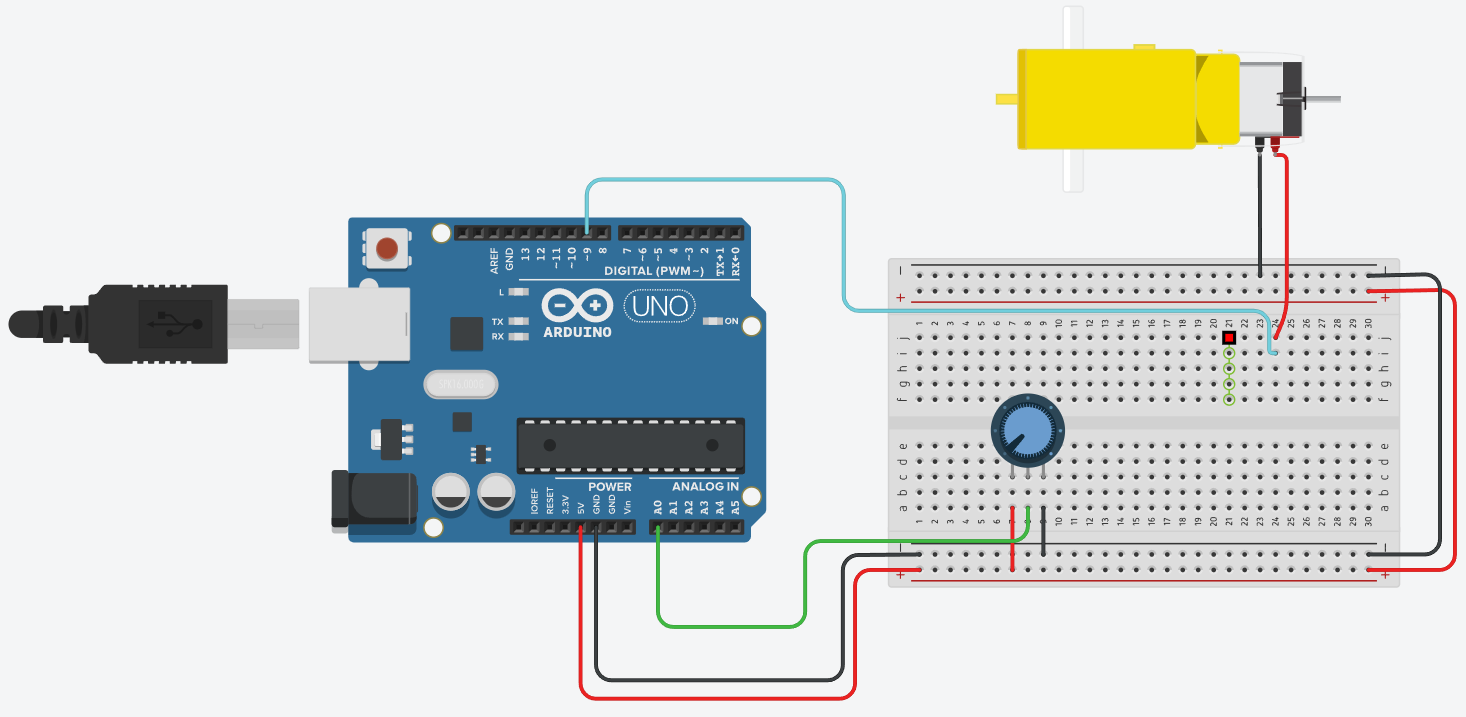
\includegraphics[width=0.85\textwidth]{./img/4-Encendido-Motor.png}
    \caption{Simulación Tinkercad Encendido de motor con Potenciometro}
    \label{fig:encendido_motor}
\end{figure}

\begin{figure}[H]
    \centering
    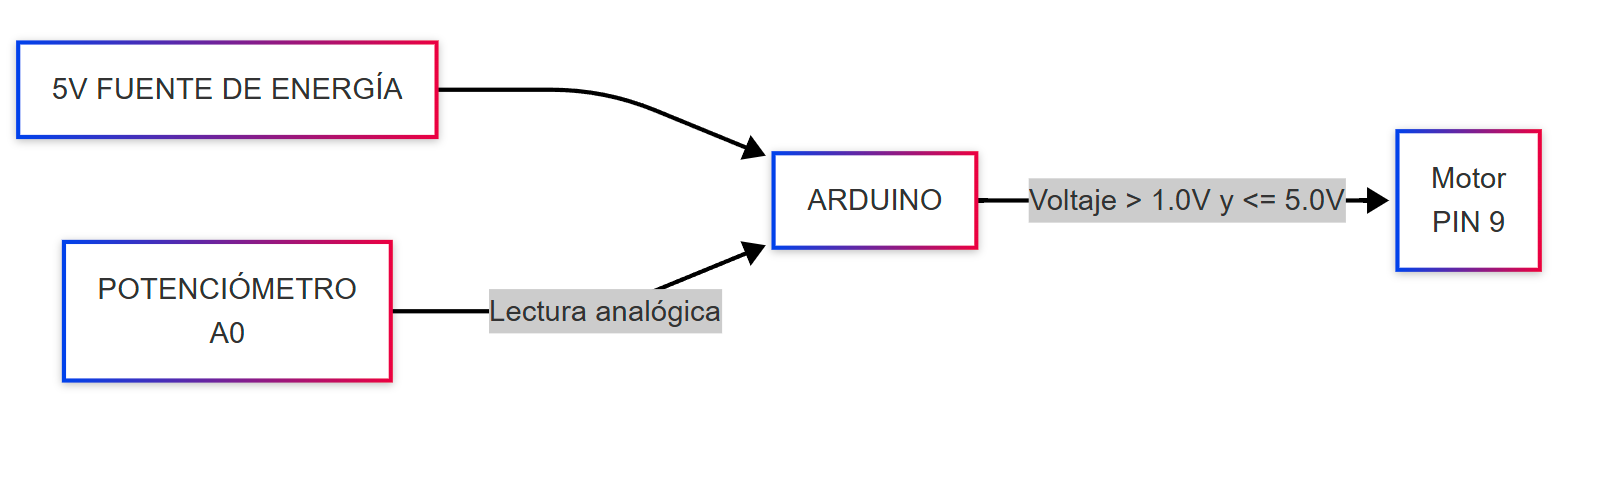
\includegraphics[width=0.85\textwidth]{./img/4-Diagrama-bloques.png}
    \caption{Diagrama de bloques del sistema de encendido de motor}
    \label{fig:bloques_encendido_motor}
\end{figure}


\begin{enumerate}
    \item ¿Qué sucede en su simulación con el Arduino?
    \item El Arduino cuando trasmite mediante el potenciometro una corriente de entre 3V y 5V segun las condiciones establecidas, el motor gira, pero con advertencia de que el voltaje puede dañar el Arduino. 
    \item ¿Cuál es la corriente que consume el motor durante su operación?
    \item El motor consume alrededor de 3.49V, esto se puede observar en la simulacion de Tinkercad.
    \item Si usted quisiera regular la velocidad del motor, ¿qué añadiría a su esquema de conexión?
    \item Para poder controlar la velocidad del motor, se puede utilizar un potenciometro o un driver de motor. El potenciometro permite regular la tension que llega al motor, mientras que el driver permite controlar la velocidad y direccion del motor.
\end{enumerate}

\section{ACTUADORES - Control de un motor con Driver}

% https://www.tinkercad.com/things/6vFVydoth82/editel?returnTo=%2Fdashboard%2Fdesigns%2Fcircuits&sharecode=zm5Em3SqUbJ5xXMONP0ul2aEuINO3AnNjSSn-egeFUc

\begin{figure}[H]
    \centering
    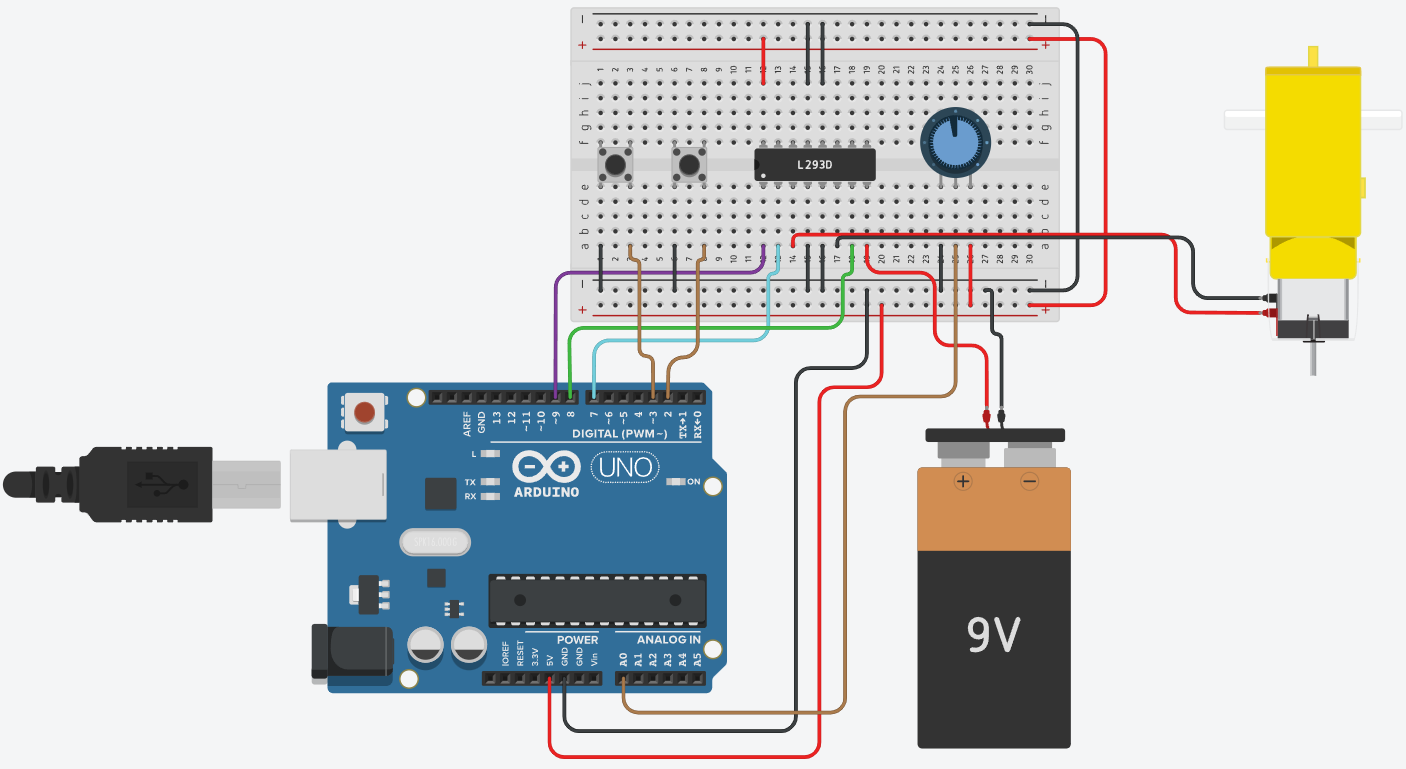
\includegraphics[width=0.85\textwidth]{./img/ckpt_motor_driver.png}
    \caption{Simulación Tinkercad ...}
    \label{fig:motor_driver}
\end{figure}

\begin{enumerate}
    \item ¿Cuál es la función del potenciómetro en este sistema de control de motor y cómo se
    relaciona con la velocidad de rotación?
    \item Explique por qué se requiere una fuente de alimentación externa para el motor en lugar de usar directamente la salida de 5V del Arduino.
    \item Describa el comportamiento esperado del motor cuando se presiona únicamente el botón
    derecho, el izquierdo, y cuando no se presiona ninguno. ¿Qué sucede si se presionan los dos?
\end{enumerate}

% TODO: simulacion
% TODO: diagrama de bloques
% TODO: respuesta a las preguntas


\section{ACTUADORES - Uso de Relé con Motor}

En esta experiencia de laboratorio se explora el uso de un módulo de relé como interfaz entre un microcontrolador (Arduino UNO o MEGA) y un motor de corriente directa (DC), permitiendo su control mediante una fuente de alimentación externa. El relé cumple un rol clave en el aislamiento eléctrico entre la etapa de control (Arduino) y la etapa de potencia (fuente y motor), lo cual es fundamental cuando se trabajan con cargas superiores a las que el microcontrolador puede manejar directamente.

Para llevar a cabo esta práctica, se utilizó un módulo de relé de un canal (5V) conectado a un Arduino. La lógica de activación del módulo es \textbf{activa en bajo}, es decir, cuando el pin de entrada IN1 recibe un nivel lógico \textbf{LOW}, el relé se activa, cerrando el circuito entre los terminales \textbf{COM} y \textbf{NO}.

El circuito se conectó de la siguiente manera:

\begin{itemize}
    \item El terminal \textbf{COM} del relé se conectó a la salida de 5V de la fuente de protoboard.
    \item El terminal \textbf{NO} del relé se conectó a uno de los terminales del motor DC.
    \item El otro terminal del motor se conectó al \textbf{GND} de la fuente de protoboard.
    \item El módulo de relé se alimentó desde el Arduino: \textbf{VCC} al pin de 5V, \textbf{GND} a tierra, e \textbf{IN1} al pin digital 7.
\end{itemize}


En la Figura~\ref{fig:rele_tinkercad} se muestra la simulación del sistema en Tinkercad, herramienta que permitió verificar el comportamiento del sistema antes de proceder a su montaje físico. La Figura~\ref{fig:rele_implementacion} presenta la implementación real del sistema sobre una protoboard, utilizando un Arduino MEGA y un módulo de relé conectado a un motor DC.


\begin{figure}[H]
    \centering
    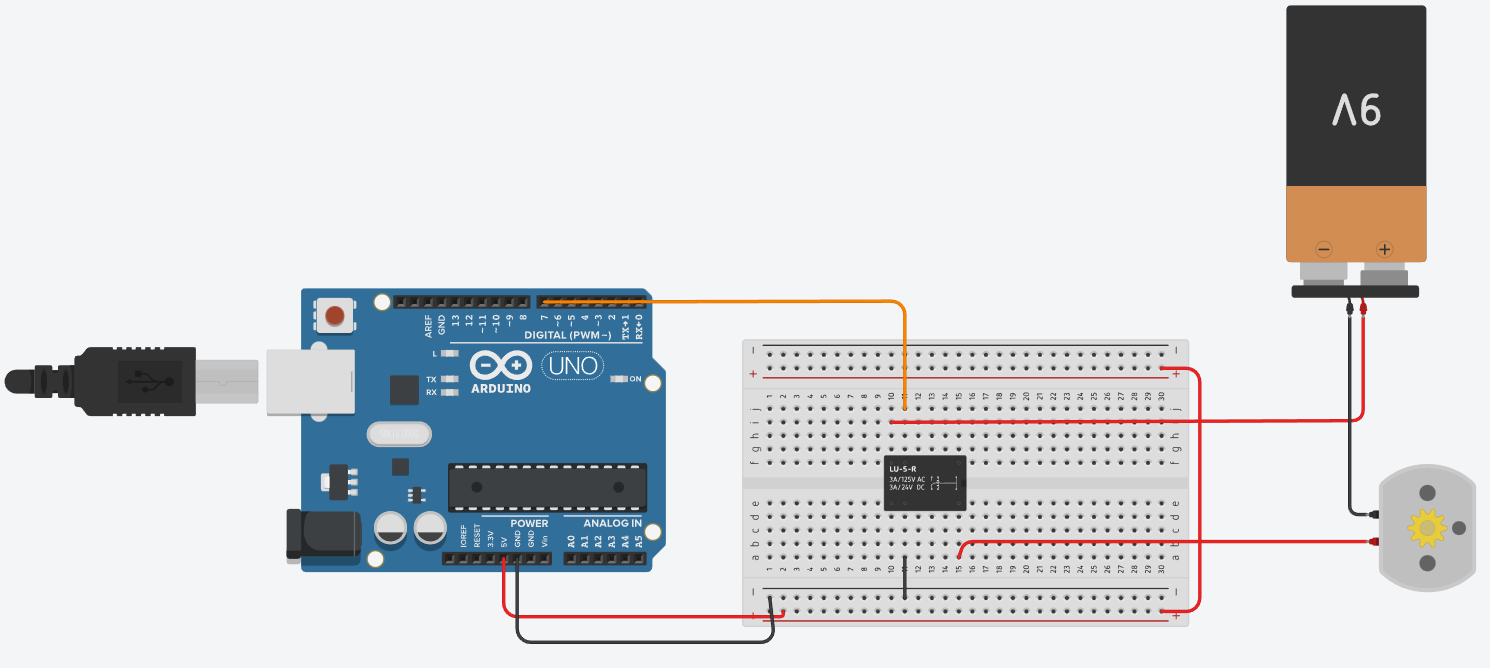
\includegraphics[width=0.85\textwidth]{./img/ckpt_rele_motor.png}
    \caption{Simulación Tinkercad}
    \label{fig:rele_tinkercad}
\end{figure}

\begin{figure}[H]
    \centering
    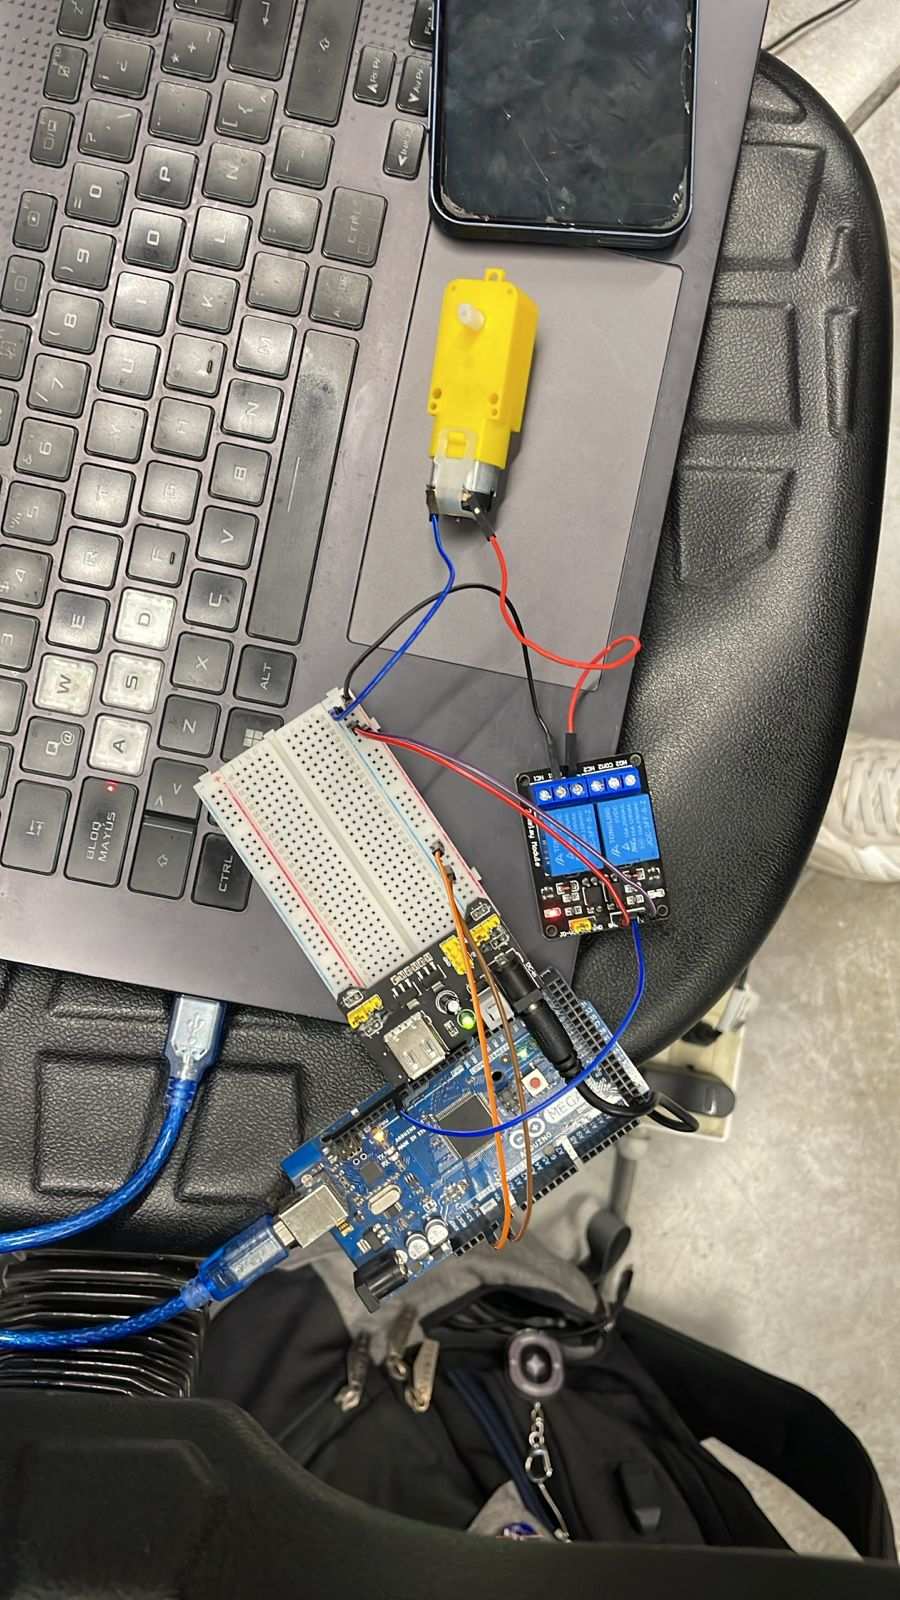
\includegraphics[width=0.5\textwidth]{./img/checkpoint_presencialrele.jpeg}
    \caption{Implementación del relé con motor}
    \label{fig:rele_implementacion}
\end{figure}

El comportamiento lógico del sistema se resume en el diagrama de flujo mostrado en la Figura~\ref{fig:flujo_rele}, donde se observa que el sistema alterna entre encender y apagar el relé (y por ende el motor) cada 5 segundos. Esta lógica fue implementada en Arduino mediante el código en C++ mostrado en el Código~\ref{code:rele_arduino}.


\begin{figure}[H]
    \centering
    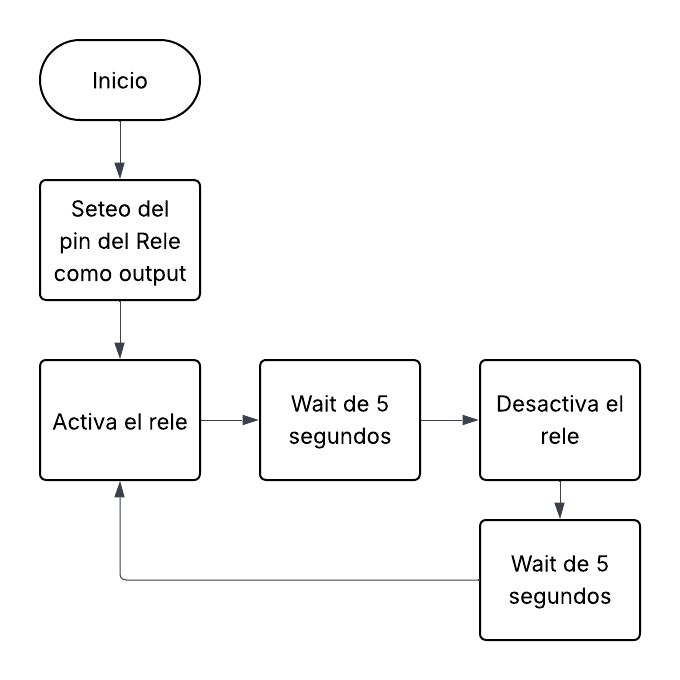
\includegraphics[width=0.5\textwidth]{./img/flujo_rele.png}
    \caption{Diagrama de flujo funcionamiento relé-motor}
    \label{fig:flujo_rele}
\end{figure}


\begin{lstlisting}[style=cppstyle, caption={Código en C++ para uso de motor con relé.}, label={code:rele_arduino}]
const int RELAY_PIN = 7;   // IN1 del modulo de rele
const int T_ON  = 3000;   // ms - tiempo encendido
const int T_OFF = 3000;   // ms - tiempo apagado

void setup() {
  pinMode(RELAY_PIN, OUTPUT);
  digitalWrite(RELAY_PIN, HIGH);   // Rele desactivado (motor OFF) al arrancar
}

void loop() {
  // Encender motor
  digitalWrite(RELAY_PIN, LOW);    // Rele activo (cierra COM-NO)
  delay(T_ON);

  // Apagar motor
  digitalWrite(RELAY_PIN, HIGH);   // Rele inactivo
  delay(T_OFF);
}
\end{lstlisting}

Finalmente, el sistema completo puede representarse con el diagrama de bloques de la Figura~\ref{fig:bloques_rele}, donde se muestra claramente la interacción entre el Arduino, el módulo de relé, la fuente de protoboard y el motor.

\begin{figure}[H]
    \centering
    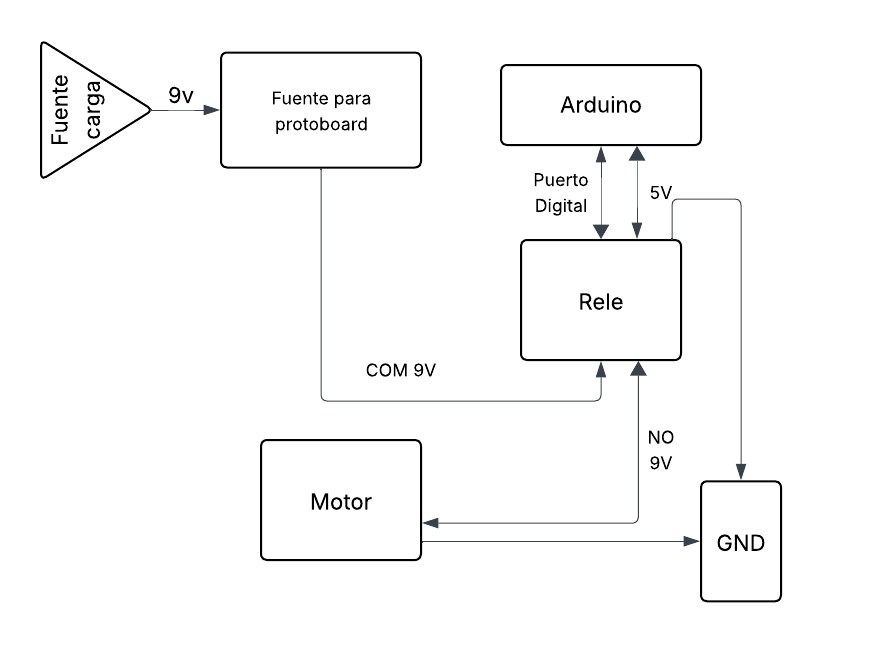
\includegraphics[width=0.75\textwidth]{./img/bloques_rele.png}
    \caption{Diagrama de bloques funcionamiento relé-motor}
    \label{fig:bloques_rele}
\end{figure}

% DONE: simulacion
% DONE: foto de la implementacion presencial en el laboratorio
% DONE: diagrama de flujo
% DONE: diagrama de bloques

\section{ACTUADORES - Uso de Driver Puente H L298N con Motor}

\begin{enumerate}
    \item Prueba alimentar el módulo L298N directamente desde el pin de 5V del Arduino (en lugar de la fuente para protoboard). ¿Notas alguna diferencia en el rendimiento del motor? Justifica técnicamente tu observación.

    Sí, se nota una disminución en el rendimiento del motor. Al alimentarlo desde el pin de 5V del Arduino, el motor se mueve más lentamente y con menos fuerza (torque). Esto ocurre porque el pin de 5V del Arduino no está diseñado para entregar grandes cantidades de corriente, y además el voltaje disponible es menor (5V frente a los 9V originales de la fuente para protoboard). Los motores DC requieren tanto un voltaje adecuado como suficiente corriente para operar eficientemente. Al reducirse estos parámetros, el motor pierde capacidad de respuesta y potencia.

    \item Restablezca la alimentación del motor. Modifica el circuito para invertir el sentido de giro automáticamente cada 3 segundos.

    Para lograr esto, se puede programar el Arduino para alternar los niveles de voltaje en los pines IN1 e IN2 del módulo L298N cada 3 segundos. Cuando IN1 está en HIGH e IN2 en LOW, el motor gira en una dirección; al invertir estos valores (IN1 en LOW e IN2 en HIGH), se invierte el sentido de giro del motor. Este cambio puede realizarse automáticamente dentro del bucle loop() del código utilizando funciones como digitalWrite() y delay(3000) para controlar el tiempo.
    
    \item ¿Qué función cumple el pin ENA en el módulo L298N y por qué debe conectarse a un pin PWM del Arduino?

    El pin ENA activa el motor A y permite controlar su velocidad. Se conecta a un pin PWM del Arduino porque estos pueden generar una señal modulada que simula un voltaje variable, lo que permite ajustar la velocidad del motor.

    \item ¿Qué sucede si se intercambian las conexiones de IN1 e IN2? ¿Cómo afecta esto a la dirección del giro del motor?

    Si se intercambian IN1 e IN2, el motor gira en sentido contrario. Esto se debe a que se invierte la polaridad de la señal que recibe el motor.

\end{enumerate}

\begin{figure}[H]
    \centering
    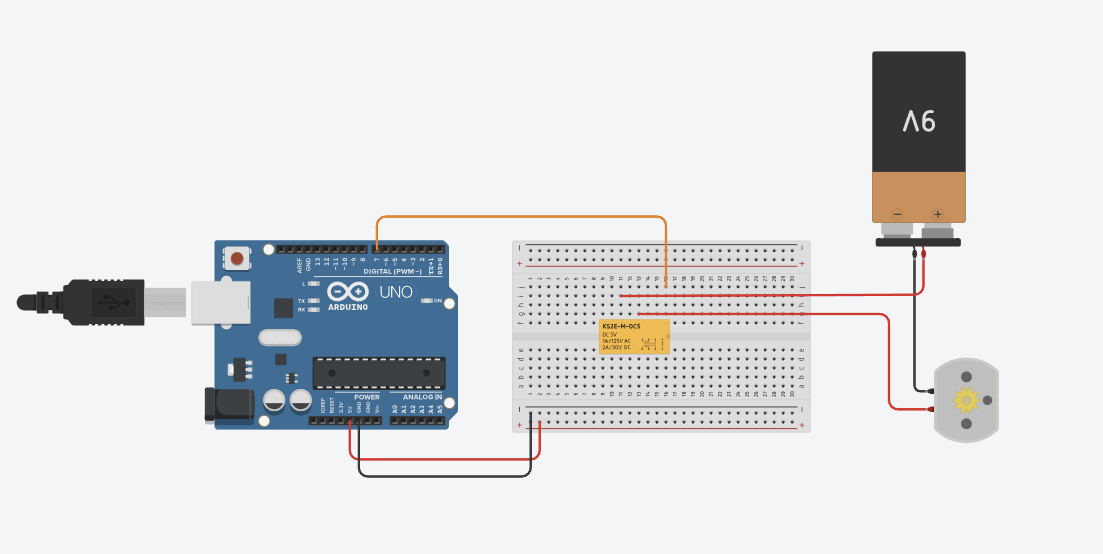
\includegraphics[width=0.85\textwidth]{./img/simulacion_puenteh.png}
    \caption{Simulación Tinkercad: Puente H L298N con Motor}
    \label{fig:l298n_simulacion}
\end{figure}

\begin{figure}[H]
    \centering
    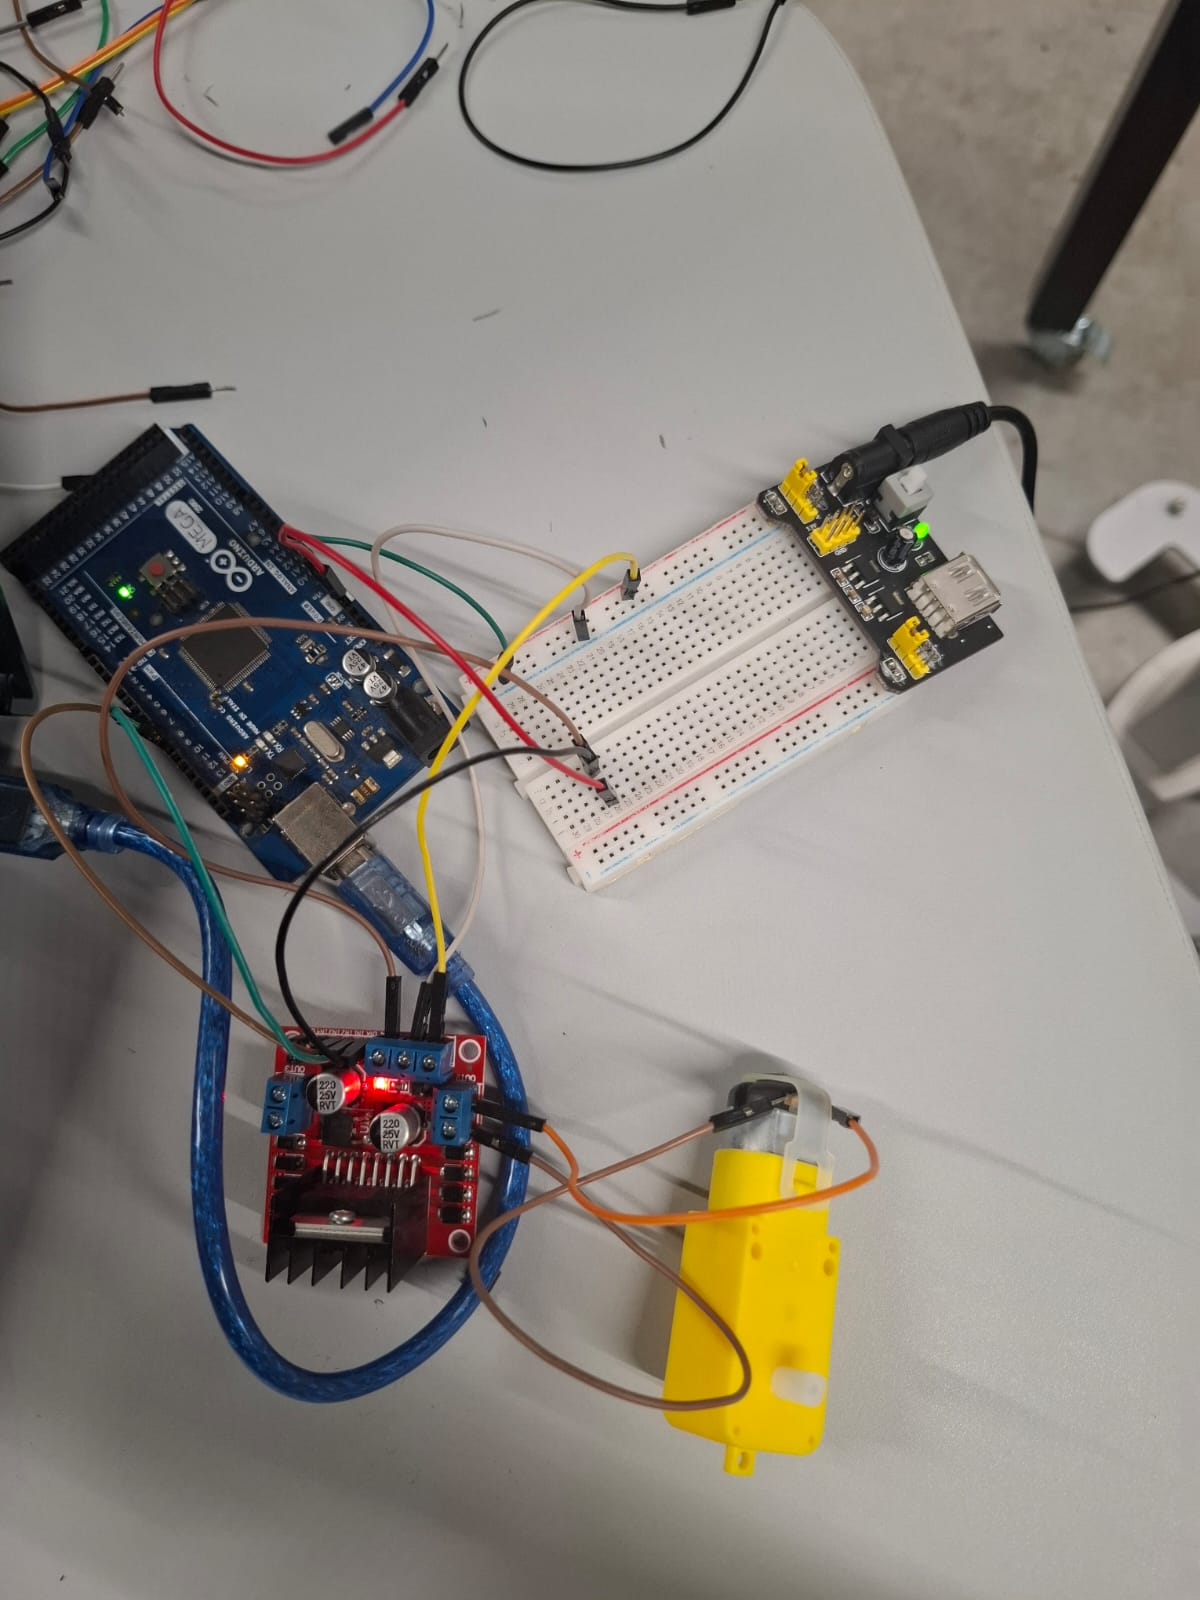
\includegraphics[width=0.65\textwidth]{./img/ckpt_presencial_298.jpeg}
    \caption{Implementación del L298N con Motor}
    \label{fig:l298n_implementacion}
\end{figure}

\begin{figure}[H]
    \centering
    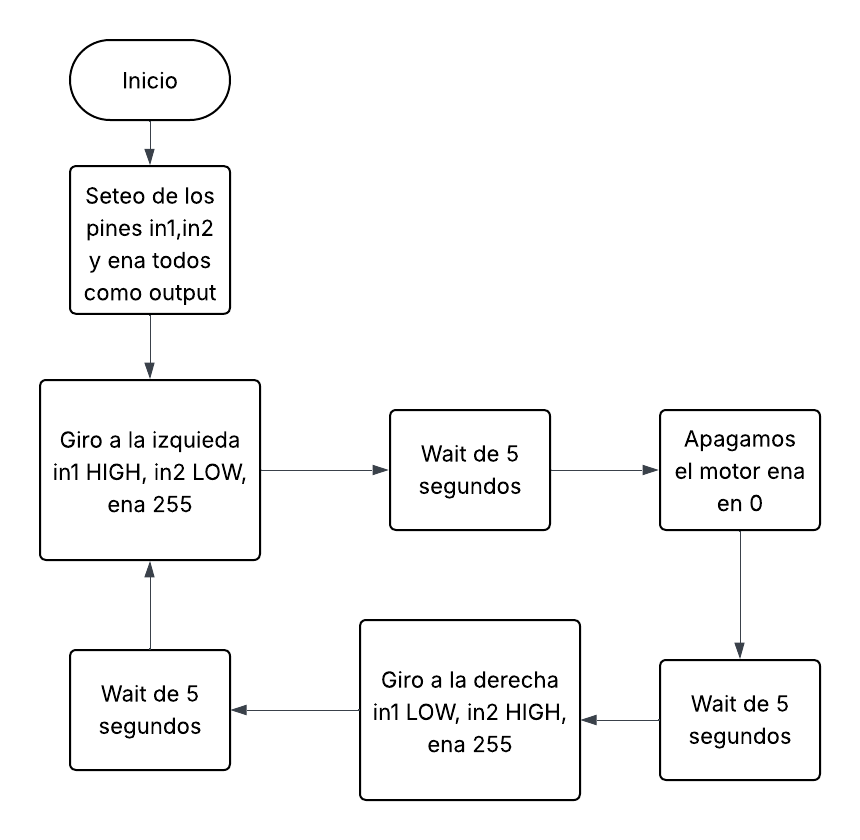
\includegraphics[width=0.7\textwidth]{./img/flujo_298.png}
    \caption{Diagrama de flujo para el L298N}
    \label{fig:flujo}
\end{figure}

\begin{figure}[H]
    \centering
    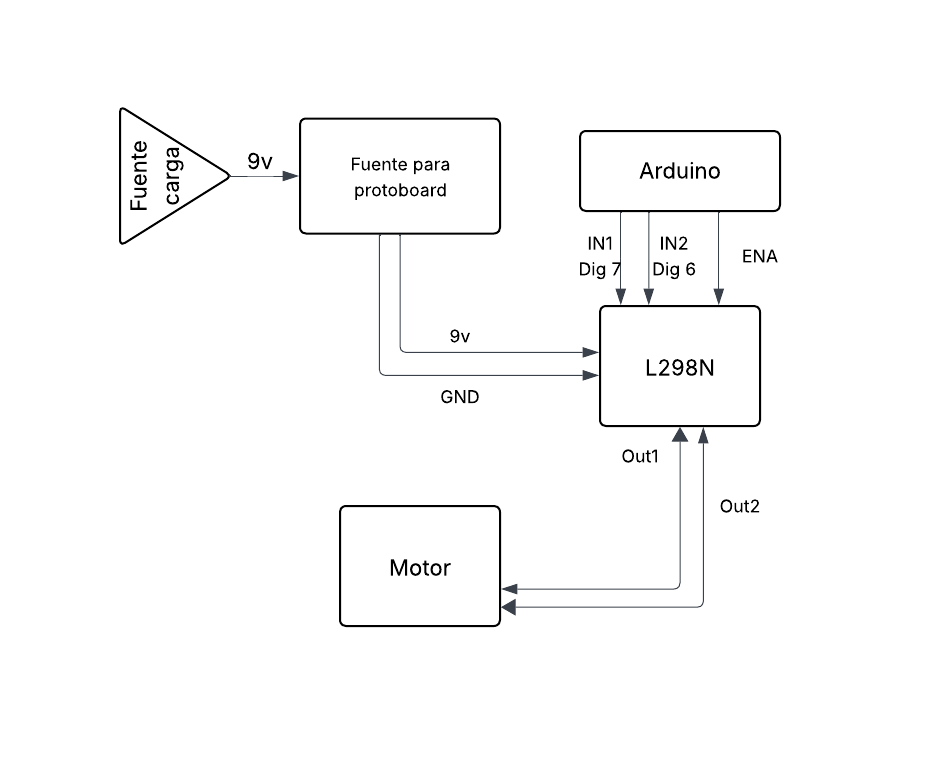
\includegraphics[width=0.65\textwidth]{./img/bloques_298.png}
    \caption{Diagrama de bloques para el L298N}
    \label{fig:bloques_l298n}
\end{figure}

% DONE: implementacion
% DONE: respuesta a las preguntas
% DONE: diagrama de flujo
% DONE: diagrama de bloques


\section{ACTUADORES - Sistema de riego inteligente}


En esta experiencia de laboratorio se desarrolló un sistema de riego automatizado que emplea un sensor de humedad de tierra para monitorear el estado del sustrato y activar una bomba de agua en función del nivel de humedad detectado. El sistema hace uso de un módulo de relé para controlar la bomba, LEDs indicadores, y un buzzer como sistema de alerta en casos de sobre-hidratación. Adicionalmente, se modificaron los hiperparámetros de umbral para el sensor de humedad con el objetivo adaptarlo a las condiciones del laboratorio, permitiendo las pruebas del sistema (Código \ref{code:riego_inteligente}).

\subsection{Componentes y Funcionamiento General}

Los componentes utilizados en el montaje se detallan a continuación:

\begin{itemize}
    \item Sensor de humedad de tierra
    \item Módulo de relé
    \item Bomba de agua
    \item LED azul (riego), LED rojo (alerta)
    \item Buzzer piezoeléctrico
    \item Arduino UNO o MEGA
\end{itemize}

El sistema opera bajo tres modos principales de funcionamiento:

\subsubsection*{1. Riego de planta}
Cuando el valor de humedad es inferior a un umbral mínimo (equivalente al 20\% de humedad), el sistema entra en estado de riego. Se activa el relé que controla la bomba de agua durante 10 segundos, y se enciende un LED azul como indicador visual. El sistema reporta en el Monitor Serial el valor de humedad y el estado actual. La Figura~\ref{fig:riego_regando} ilustra este estado en la implementación real.

\subsubsection*{2. Estado IDLE}
Después de regar la planta, el sistema entra en un estado de reposo durante 15 segundos. Durante este tiempo, no se hacen nuevas mediciones ni se activa la bomba. El Monitor Serial muestra el mensaje “Modo IDLE”. Ver Figura~\ref{fig:riego_logs}.

\subsubsection*{3. Estado de alerta}
Si el nivel de humedad supera el 75\%, el sistema considera que la planta está sobre-hidratada. En este caso, se activa una alarma sonora (buzzer) y visual (LED rojo intermitente), ambos operando de forma parpadeante para llamar la atención. La Figura~\ref{fig:riego_sobrehidratacion} muestra este estado en la implementación.

La Figura~\ref{fig:bloques_riego_inteligente} muestra el diagrama de bloques general del sistema, donde se observa la interacción entre los sensores, actuadores y la unidad de control. A continuación, se incluye el código completo implementado para gestionar los estados y componentes.

\begin{figure}[H]
    \centering
    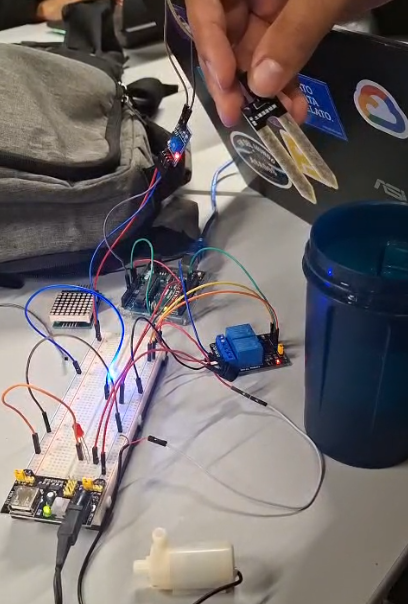
\includegraphics[width=0.4\textwidth]{./img/riego_estado_riego.png}
    \caption{Implementación en laboratorio: Estado de riego (LED azul encendido)}
    \label{fig:riego_regando}
\end{figure}

\begin{figure}[H]
    \centering
    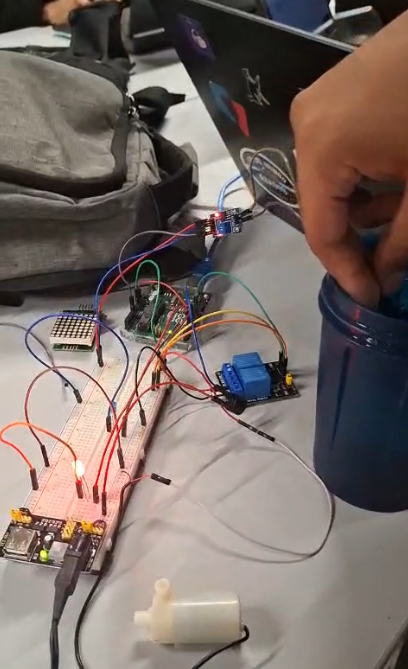
\includegraphics[width=0.4\textwidth]{./img/riego_sobrehidratacion.png}
    \caption{Implementación en laboratorio: Estado de alerta (LED rojo intermitente y buzzer activo)}
    \label{fig:riego_sobrehidratacion}
\end{figure}


\begin{figure}[H]
    \centering
    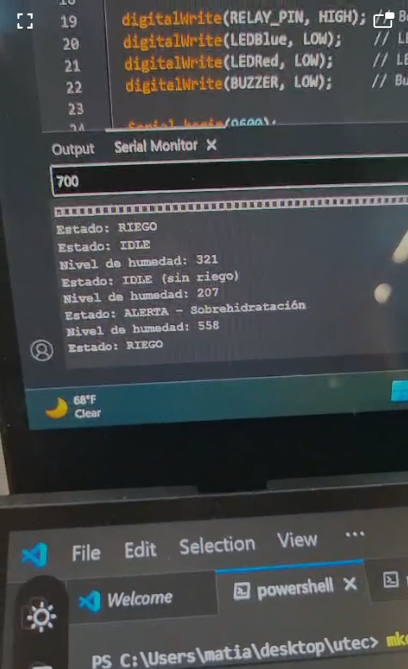
\includegraphics[width=0.4\textwidth]{./img/riego_monitoreo.png}
    \caption{Implementación en laboratorio: Logs del sistema}
    \label{fig:riego_logs}
\end{figure}


\begin{figure}[H]
    \centering
    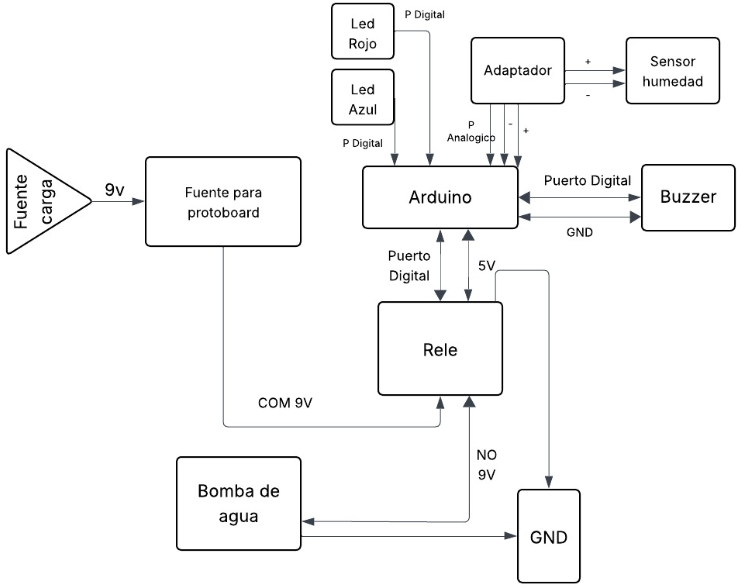
\includegraphics[width=0.7\textwidth]{./img/bloques_riego_inteligente.png}
    \caption{Diagrama de bloques para el sistema de riego inteligente}
    \label{fig:bloques_riego_inteligente}
\end{figure}

\begin{lstlisting}[style=cppstyle, caption={Código en C++ para sistema de riego inteligente con relé.}, label={code:riego_inteligente}]
int RELAY_PIN = 10;    // Rele para bomba
const int LEDBlue = 7; // LED azul (riego)
const int LEDRed = 4;  // LED rojo (alerta)
const int BUZZER = 5;  // Buzzer de alerta
int SensorPin = A0;    // Sensor de humedad

const int t_riego = 10000; // 10 segundos riego
const int t_idle = 15000;  // 15 segundos IDLE

const int umbral_riego = 700;   // 20% humedad (ajustar segun sensor)
const int umbral_alerta = 300;  // 75% humedad (ajustar segun sensor)

void setup() {
  pinMode(RELAY_PIN, OUTPUT);
  pinMode(LEDBlue, OUTPUT);
  pinMode(LEDRed, OUTPUT);
  pinMode(BUZZER, OUTPUT);

  digitalWrite(RELAY_PIN, HIGH); // Bomba OFF
  digitalWrite(LEDBlue, LOW);    // LED azul OFF
  digitalWrite(LEDRed, LOW);     // LED rojo OFF
  digitalWrite(BUZZER, LOW);     // Buzzer OFF

  Serial.begin(9600);
}

void loop() {
  int humedad = analogRead(SensorPin);

  Serial.print("Nivel de humedad: ");
  Serial.println(humedad);

  if (humedad <= umbral_riego) {
    // Estado de Riego
    Serial.println("Estado: RIEGO");

    digitalWrite(LEDBlue, HIGH);  // LED Azul ON
    digitalWrite(RELAY_PIN, LOW); // Bomba ON
    delay(t_riego);

    // Pasar a modo IDLE
    Serial.println("Estado: IDLE");

    digitalWrite(RELAY_PIN, HIGH); // Bomba OFF
    digitalWrite(LEDBlue, LOW);    // LED Azul OFF
    delay(t_idle);

  } else if (humedad >= umbral_alerta) {
    // Estado de Alerta
    Serial.println("Estado: ALERTA - Sobrehidratacion");

    for (int i = 0; i < 5; i++) {  // 5 parpadeos
      digitalWrite(LEDRed, HIGH);
      digitalWrite(BUZZER, HIGH);
      delay(500);

      digitalWrite(LEDRed, LOW);
      digitalWrite(BUZZER, LOW);
      delay(500);
    }

  } else {
    // Estado IDLE normal
    Serial.println("Estado: IDLE (sin riego)");

    digitalWrite(RELAY_PIN, HIGH); // Bomba OFF
    digitalWrite(LEDBlue, LOW);    // LED Azul OFF
    digitalWrite(LEDRed, LOW);     // LED Rojo OFF
    digitalWrite(BUZZER, LOW);     // Buzzer OFF
    delay(1000); // Pausa para lecturas
  }
}
\end{lstlisting}


% DONE: foto de la implementacion presencial en el laboratorio
% TODO: diagrama de flujo
% DONE: diagrama de bloques


\section{ACTUADORES - Control de ventiladores}

% TODO: solo simulacion Tinkercad
% TODO: diagrama de bloques del sistema